%%%%%%%%%%%%%%%%%%%%%%%%%%%%%%%%%%%%%%%%%%%%%%%%%%%%%%%%%%%%%%%%%%%%%%%%%%%%%%%%%%%%%%%%%%
%%%  EKAW 2016 - DOREMUS to Schema.org: Mapping a Complex Vocabulary to a Simpler One  %%%
%%%%%%%%%%%%%%%%%%%%%%%%%%%%%%%%%%%%%%%%%%%%%%%%%%%%%%%%%%%%%%%%%%%%%%%%%%%%%%%%%%%%%%%%%%

\documentclass{llncs}

\usepackage{url}
\usepackage{graphicx}
\usepackage{xtab}
\usepackage[inline]{enumitem}
\usepackage[title]{appendix}
\DeclareGraphicsExtensions{.png}

%%%%%%%%%%%%%%%%%%%%%%%%%%%%%%%
%%%  Beginning of document  %%%
%%%%%%%%%%%%%%%%%%%%%%%%%%%%%%%

\begin{document}

\title{DOREMUS to Schema.org: Mapping a Complex Vocabulary to a Simpler One}

\author{Pasquale Lisena\inst{1} \and Rapha\"el Troncy\inst{1}}
\authorrunning{Lisena and Troncy}
\institute{EURECOM, Sophia Antipolis, France \\
\email{\{pasquale.lisena|raphael.troncy\}@eurecom.fr}}

\maketitle

%%%%%%%%%%%%%%%%%%
%%%  Abstract  %%%
%%%%%%%%%%%%%%%%%%

\begin{abstract}
Librarians and music professionals often us complex models and ontologies such as FRBRoo to represent music metadata. As a consequence, this metadata is not easily consumable by general search engines or external web applications. This paper presents a methodology, composed of a set of recipes, for mapping a complex ontology to a simpler model, namely Schema.org.

%\keywords{Ontology, FRBRoo, Music Metadata, Schema.org}
\end{abstract}

%%%%%%%%%%%%%%%%%%%%%%%%%%%%%%%%%%%%%%%%%%%%%%%%%%
%%%  1. Music Information and Structured Data  %%%
%%%%%%%%%%%%%%%%%%%%%%%%%%%%%%%%%%%%%%%%%%%%%%%%%%

\section{Music Information and Structured Data}
\label{sec:introduction}
Search engines and web applications display more and more knowledge panels alongside raw search results. This is made possible thanks to the adoption of some form of \textit{Structured Data markup}, like Schema.org \cite{guha2015schema} that allows to describe the content of a web page in a machine-understandable way. In particular, Schema.org offers classes such as \texttt{CreativeWork} or \texttt{Event} and music-specific subclasses such as \texttt{MusicComposition} or \texttt{MusicEvent}.

Musical works are complex objects that require complex ontologies for expressing the richness of the information. FRBRoo is an ontology for describing bibliographic information~\cite{doerr2008frbroo}. The central feature of this ontology is the presence of the triplet Work-Event-Expression which considers that any artistic Work, only exists through an Event of creation, that realizes the Work itself into an Expression. The DOREMUS ontology\footnote{\url{http://www.doremus.org}}~\cite{achichidoremus} extends FRBRoo with music-specific classes and properties like the key, the genre or the casting that could interpret a work. Because of this complexity, the consumption of these data by search engines and external applications is not easy.
Nogales et al. proposed a mapping between the classes and properties of Schema.org and the ones of different vocabularies which have exactly the same name (or synonyms)~\cite{nogales2016linking}. Godby proposes to map each level of the chain Work - Expression - Manifestation - Item with a entity of the CreativeWork class~\cite{godby2013relationship}. A limit of this strategy is that the information is split up among different objects.

In this paper, we provide a methodology composed of four recipes for translating a complex ontology like DOREMUS into Schema.org. This method is based on the observation of the graph and it assumes sufficient knowledge of the source and target models. As example, we will represent Beethoven's \textit{Sonata ``Quasi una Fantasia''}, described in DOREMUS in Figure~\ref{fig:beet-doremus} using Schema.org\footnote{In the following we use respectively the prefixes \texttt{mus:} and \texttt{sdo:}}.

\begin{figure}
 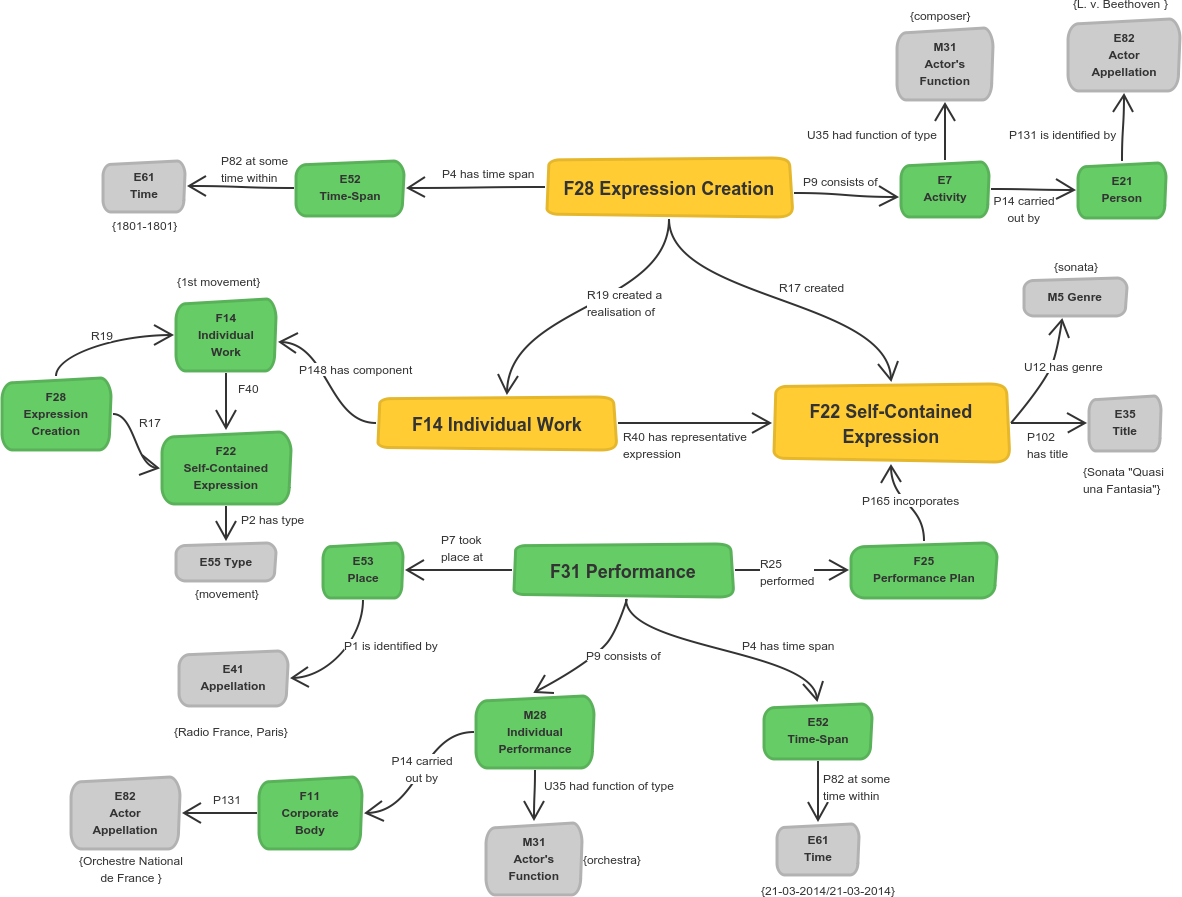
\includegraphics[width=11cm]{img/Beethoven-Doremus.png}
 \centering
 \caption{Graph describing Beethoven's \textit{Sonata ``Quasi una Fantasia"} in DOREMUS.}
 \label{fig:beet-doremus}
\end{figure}

%%%%%%%%%%%%%%%%%%%%%%%%%%%%%%%%%
%%%  2. Model Simplification  %%%
%%%%%%%%%%%%%%%%%%%%%%%%%%%%%%%%%

\section{Model Simplification}
\label{sec:simplification}

\subsubsection{Choose the starting node.}
The most suitable starting point should coincide with the most significant class (or group of classes) in the source ontology (e.g. DOREMUS). It could be the class with the biggest number of instances, or it could consist in a frequent pattern, like the FRBRoo triangle. We choose \textit{mus:F2 Expression} and \textit{mus:F28 Expression Creation}, because they are linked with most of the crucial information for end-users such as the title and the composer.

\subsubsection{Identify similar classes.}
\label{sec:classmap}
For each class in DOREMUS, the best match in Schema.org should satisfy one or more of these criteria:
\begin{enumerate*}
 \item Have similar names, where similarity is computed using the Levenshtein distance or the number of common synonyms;
 \item Have similar descriptions, where the similarity can be computed using the cosine or a Token-Wise distance;
 \item Have similar properties;
 \item Have similar expected property values (e.g. both \texttt{mus:U12\_has\_genre} and \texttt{sdo:musicCompositionForm} have ``sonata'' as possible value).
\end{enumerate*}
If the search for a suitable match fails for a specific class, then it could mean that such an equivalent concept does not exist in Schema.org. In this case, this information can either be considered as too specific to be mapped or represented in a plain text note. Alternatively, new classes and properties could be considered in Schema.org extensions.

\subsubsection{Identify similar properties.}
For each class mapped, we must align their properties. The criteria are again: have similar names, have similar descriptions and have similar expected values. Each mapped property could have as value a literal (e.g. key and genre) or another class (e.g. the composer is a Person). In the latter case, if we have not previously mapped it, we consider this class as a new input for the first steps, until every node in the graph is reached.

\subsubsection{Simplify the graph.}
Different DOREMUS classes can be mapped to the same Schema.org type: e.g. both Works and Expressions are mapped to \texttt{sdo:Music\-Composition}. Merging these nodes can produce the advantage of a simpler model, in which the information is distributed in as less nodes as possible. Two nodes are good candidates for the merging when:
\begin{enumerate*}
 \item They have the class or a superclass in common;
 \item The direct connection with a specific class is realized with the same property;
 \item They are directly connected;
 \item They have no conflicting properties.
\end{enumerate*}
The \texttt{mus:F1\_Work} and \texttt{mus:F2\_Expression} classes aligned with \texttt{sdo:MusicComposition} satisfy all these criteria. The difference between Work and Expression as defined by FRBRoo has also been considered as tiny from the point of view of Schema.org~\cite{godby2013relationship}.

Redundant nodes are substituted with a new node with:
\begin{enumerate*}
\item The same class of the original one (or the most specific among the two);
\item The sum of their properties.
\end{enumerate*}
The result of this phase is a new graph as depicted in Figure~\ref{fig:beet-schema}.

\begin{figure}
 \centering
 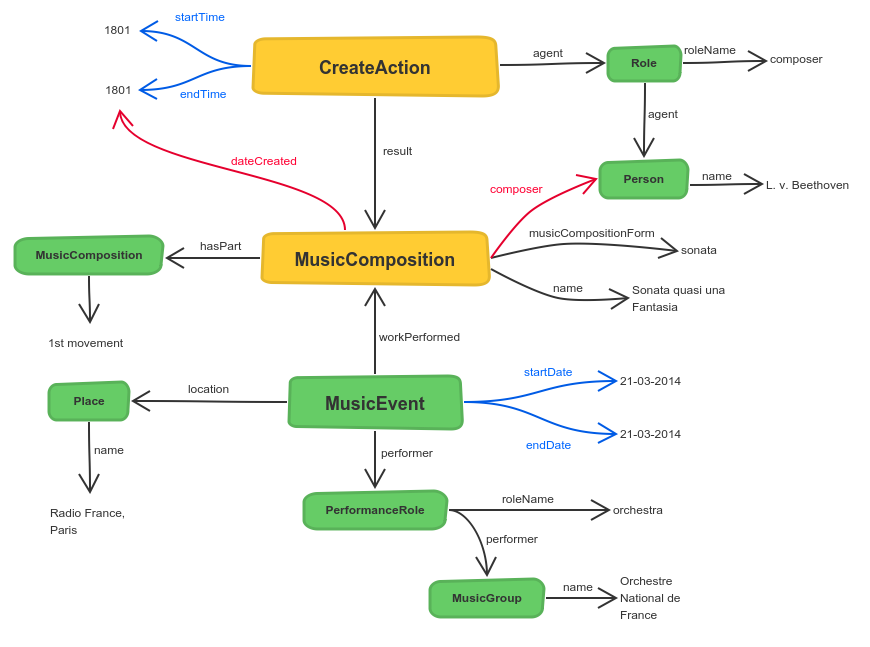
\includegraphics[width=11cm]{img/Beethoven-Schema.png}
 \caption{Graph of Beethoven's \textit{Sonata ``Quasi una Fantasia''} in Schema.org.}
 \label{fig:beet-schema}
\end{figure}

%%%%%%%%%%%%%%%%%%%%%%%%%%%%%%%%%%%%%%%
%%%  3. Evaluation and Future Work  %%%
%%%%%%%%%%%%%%%%%%%%%%%%%%%%%%%%%%%%%%%

\section{Evaluation and Future Work}
\label{sec:evaluation}
The evaluation of the goodness of the mapping is a long term goal, that can be realized only when data will be more easily consumed (e.g. by search engines). For having a quick feedback, we prepared a JSON-LD version of the \textit{Sonata Quasi Una Fantasia} available at \url{https://goo.gl/zzXVVh}.
Both the Structured Data Testing Tool by Google\footnote{\url{https://search.google.com/structured-data/testing-tool}} and the Structured Data Linter\footnote{\url{http://linter.structured-data.org/}} show the structure of the Schema.org graph like a tree, with 76 statements correctly recognized. The Structured Data Linter offers in addition a preview of the result as they could be shown in a SERP. For having a stronger visual feedback, we developed a lightweight web application, named \emph{Schema.org Visualizer}\footnote{\url{https://github.com/pasqLisena/schema-visualizer}}, which consumes the data in JSON-LD and shows a knowledge cards for the described content. The result for our example is available at \url{https://goo.gl/mCAszw}.

We are planning to test our recipes on the ELI ontology\footnote{\url{http://publications.europa.eu/mdr/eli/}} which is also based on FRBRoo. The goal is to compare the result of the mapping to the one which has recently been hand-made designed for being considered as a Schema.org extension\footnote{\url{https://github.com/schemaorg/schemaorg/issues/1156}}. Future work includes an implementation strategy for this methodology, that will also highlight the content excluded from the mapping, in order to better evaluate the possibility of presenting a Schema.org extension.

\subsubsection*{Acknowledgments.}
This work has been partially supported by the French National Research Agency (ANR) within the DOREMUS Project, under grant number ANR-14-CE24-0020.

% ---- Bibliography ----
\bibliographystyle{abbrv}
\bibliography{bib-doremus}

\newpage

\end{document} 